\section{Evaluation and Benchmarking}
\label{sec:evaluation_benchmarking}

This section is a meta-evaluation of Speech LLM benchmarks rather than a
catalog. We ask three questions: what current benchmarks measure, how
reliably they measure it, and what remains invisible to them. Building on
text-LLM evaluation efforts such as HELM, MMLU, and BIG-Bench
\cite{liang2022helm,hendrycks2021measuring,srivastava2023beyond}, we identify
the speech-specific extensions that an IPM-quality survey must demand.

\subsection{From LLM Evaluation to Speech LLM Evaluation}
\label{subsec:eval_setup}

Evaluation is where claims about Speech LLM training become claims about
capability, reliability, and deployability. Classical machine learning
organizes evaluation around three elements: a dataset, a protocol, and a
metric. LLM evaluation complicates all three. Open-ended generation weakens
single-label scoring \cite{liang2022helm}, prompt and decoding choices
introduce non-trivial score variance \cite{hendrycks2021measuring},
training-data contamination is difficult to rule out
\cite{srivastava2023beyond}, and LLM-as-judge protocols create a circular
dependency in which the evaluator itself becomes an object of evaluation
\cite{zheng2023judging}.

Speech adds another layer of difficulty. A speech input is not a text
sequence but a \emph{multi-channel acoustic signal} carrying linguistic
content, paralinguistic information, speaker traits, accent, acoustic
scene, timing, and interaction dynamics simultaneously. Word error rate,
BLEU, exact match, and MOS-style scores are therefore necessary but
incomplete: each observes only a slice of speech behavior. A system can
transcribe words correctly while missing emotion, produce a semantically
plausible answer while ignoring background events, or generate a correct
response too late for natural conversation. Recent benchmarks expose these
failures from different angles:

\begin{itemize}
  \item \textbf{Acoustic--semantic misalignment}: SALMon \cite{maimon2024salmon} probes whether models bind acoustic context to spoken content.
  \item \textbf{Fine-grained paralinguistic blindness}: FMSU-Bench \cite{li2026fmsubench} and VoxEmo \cite{zhang2026voxemo} expose weaknesses in micro-acoustic perception.
  \item \textbf{Multilingual and code-switching fragility}: Dynamic-SUPERB \cite{huang2024dynamicsuperb} and SCENEBench \cite{iyer2026scenebench} include explicit cross-lingual stress cases.
  \item \textbf{Interaction instability}: StyleBench \cite{zhao2026stylebench} and VoiceAgentBench \cite{jain2025voiceagentbench} target multi-turn behavior and tool use.
  \item \textbf{Cross-modal safety divergence}: VoiceBench \cite{chen2024voicebench} shows that safety responses can change between text and speech modes; we develop this further in Section~\ref{sec:safety_privacy_governance}.
\end{itemize}

The question for evaluation is therefore not only whether a model performs
well on a task, but whether the benchmark measures the speech-specific
behavior that matters for real use. Subsequent subsections audit whether
current benchmarks meet that bar.

\subsection{Benchmark Corpus and Scope}
\label{subsec:eval_corpus}

We analyze 18 benchmarks from 2024--2026 that evaluate speech-relevant
capabilities of LLM-based systems. The pool includes benchmarks designed
directly for Speech LLMs, broader Audio LLM benchmarks when their tasks
transfer to speech interaction (judged by whether at least half their
prompts contain spoken language as primary signal), and voice-assistant,
agentic, multilingual, paralinguistic, and auditory-knowledge benchmarks
when they evaluate speech-relevant behavior. Traditional ASR and TTS
benchmarks are used only as background unless embedded in a Speech LLM
evaluation protocol. Of the 18 benchmarks, 3 are peer-reviewed
(SD-Eval at the NeurIPS 2024 Datasets and Benchmarks track \cite{ao2024sdeval}, Dynamic-SUPERB at ICLR 2025
\cite{huang2024dynamicsuperb},
SLUE-PERB at INTERSPEECH 2023 \cite{shon2023slue}); the remaining 15 are
arXiv preprints as of June 2026 (we count only benchmarks with confirmed
proceedings or journal publication, not papers under review). We label
preprint evidence as such throughout and avoid claims that depend on
un-peer-reviewed sample sizes or rankings.

For Figure~\ref{fig:benchmark_heatmap}, we coded capability coverage as
a binary indicator: a dimension is counted when the benchmark
explicitly defines a task, supplies test data, and reports a metric for
that dimension; partial or implicit coverage was not counted.
Disagreements during coding were resolved by re-reading the original
paper rather than by inference.

\paragraph{Search and selection.}
Benchmarks were identified via Google Scholar, the arXiv
\texttt{cs.CL} and \texttt{eess.AS} categories, the ACL Anthology, and
the proceedings of NeurIPS, ICLR, ICML, INTERSPEECH, and ICASSP,
covering January 2024 through June 2026. We searched for
``Speech LLM'', ``Audio LLM'', ``voice assistant benchmark'', ``speech
evaluation'', ``audio jailbreak'', ``full-duplex speech'', and
``streaming speech model''. A benchmark was included when it evaluated
an LLM-based system on speech or audio input, defined tasks with test
data and metrics, and covered at least one capability dimension from
Figure~\ref{fig:benchmark_heatmap}; pure ASR or TTS benchmarks were
excluded unless they were embedded in a Speech LLM evaluation protocol.
Coding for Figure~\ref{fig:benchmark_heatmap} was performed by a single
reviewer with disagreements resolved by re-reading the source paper
rather than by inference; per-benchmark reading notes are released as
supplementary material so that the coding can be independently
validated by the community. We label this corpus as a 2024--2026
snapshot; given that fifteen of the eighteen benchmarks were arXiv
preprints at the time of writing, some entries may have been
peer-reviewed or superseded by the time of publication, and the
analysis should be read as a contemporaneous audit rather than a final
record.

\subsection{A Two-Axis Taxonomy of Speech LLM Benchmarks}
\label{subsec:eval_taxonomy}

A single-axis taxonomy by task family is useful but insufficient. The same
benchmark can be broad in modality coverage, narrow in evaluation lens, and
partially anchored to a deployment use case. We organize the benchmark
landscape using two orthogonal axes. The \emph{scope} axis describes
breadth and depth: targeted probe, capability-focused suite, holistic
suite, or use-case-grounded evaluation. The \emph{lens} axis describes the
benchmark's dominant evaluative perspective: capability, use case,
phenomenon, or knowledge. Table~\ref{tab:benchmark_taxonomy} shows primary
placements with secondary lenses noted in footnotes; placements are not
exclusive. VoiceBench is use-case-grounded but also probes robustness and
safety; SCENEBench is primarily phenomenon-oriented but has use-case
flavor; FMSU-Bench can be read as both capability-focused and a targeted
paralinguistic probe.

We read Table~\ref{tab:benchmark_taxonomy} by row first (scope) and then by
column (lens). Cells with multiple entries indicate saturation of
attention; empty cells indicate evaluation blind spots.
\begin{table}[t]
\centering
\caption{Primary placement of 18 Speech LLM benchmarks (2024--2026) under a
scope $\times$ lens taxonomy.}
\label{tab:benchmark_taxonomy}
\scriptsize
\setlength{\tabcolsep}{4pt}
\renewcommand{\arraystretch}{1.18}

\begin{threeparttable}
\begin{tabularx}{\textwidth}{
  >{\RaggedRight\arraybackslash\bfseries}p{0.13\textwidth}
  Y Y Y Y
}
\toprule
Scope / Lens & Capability & Use case & Phenomenon & Knowledge \\
\midrule

Targeted probe
&
SALMon (8 tasks)\cite{maimon2024salmon};
VoxEmo (35 corpora)\cite{zhang2026voxemo};
StyleBench (4 dims)\cite{zhao2026stylebench};
SD-Eval\tnote{$\dagger$} (4 dims, 7.3K)\cite{ao2024sdeval}
&
\na
&
LoASR-Bench (25 langs)\cite{chen2026loasrbench};
Hearing2Translate (16 benchmarks)\cite{papi2025hearing2translate};
SCENEBench\tnote{$\ddagger$} (4 tasks)\cite{iyer2026scenebench}
&
AKB-2000 (2K Q)\cite{lu2026akb2000}
\\
\addlinespace[0.35em]

Capability-focused
&
AudioBench (26 datasets, 100K+)\cite{wang2025audiobench};
AIR-Bench (19 tasks, 19K+)\cite{yang2024airbench};
FMSU-Bench\tnote{$\star$} (14 dims, 20K)\cite{li2026fmsubench};
SeaLLMs-Audio (1.58M train, 580 test)\cite{liu2025seallmsaudio}
&
\na
&
\na
&
\na
\\
\addlinespace[0.35em]

Holistic
&
Dynamic-SUPERB\tnote{$\dagger$} (180 tasks)\cite{huang2024dynamicsuperb};
MMAU (10K Q, 27 skills)\cite{sakshi2024mmau}
&
\na
&
\na
&
\na
\\
\addlinespace[0.35em]

Use-case-grounded
&
\na
&
VoiceBench\tnote{$\star$} (8 tasks, 3K)\cite{chen2024voicebench};
VoiceAgentBench (6 tasks, 6K)\cite{jain2025voiceagentbench};
Audio2Tool (8 tiers, 30K)\cite{pahwa2026audio2tool};
SLUE-PERB\tnote{$\dagger$} (4 tasks, 22K)\cite{shon2023slue}
&
\na
&
\na
\\

\bottomrule
\end{tabularx}

\begin{tablenotes}[flushleft]
\footnotesize
\item \textit{Notes.} Scale denotes total samples, rounded when reported.
\item[$\dagger$] Peer-reviewed.
\item[$\star$] Capability-focused secondary lens.
\item[$\ddagger$] Use-case-grounded secondary lens.
\end{tablenotes}
\end{threeparttable}
\end{table}
The matrix exposes three structural gaps:

\begin{itemize}
  \item \textbf{The empty Use-case $\times$ Capability cell.} No benchmark
  in our corpus of 18 asks whether a model can complete a realistic job
  \emph{while} preserving a specific speech capability such as emotion
  awareness, code-switching fidelity, or robust tool calling under
  noise. A practitioner cannot select a Speech LLM for a real-time
  multilingual emotional assistant by reading benchmark scores.
  \item \textbf{Sparse Knowledge lens.} AKB-2000 \cite{lu2026akb2000} is
  the only benchmark in our corpus that systematically probes what
  auditory knowledge the LLM backbone encodes, despite backbone choice
  being a first-order Speech LLM design decision.
  \item \textbf{Narrow Phenomenon lens.} Multilinguality, translation, and
  acoustic-scene conditions are well represented (LoASR-Bench,
  Hearing2Translate, SCENEBench), but privacy, safety, latency, and
  interaction phenomena remain weakly integrated into mainstream
  benchmark design.
\end{itemize}

Beyond the structural placement of benchmarks, we now ask which
capabilities they collectively measure.

\subsection{What Current Benchmarks Actually Measure}
\label{subsec:eval_coverage}

The bar chart in Figure~\ref{fig:benchmark_heatmap} summarizes 18
benchmarks across 17 capability dimensions (the full 18~$\times$~17
binary matrix is released as supplementary material). We group
capabilities into three tiers by frequency.

\paragraph{Saturated capabilities ($\geq$10/18).}
ASR/transcription, speech QA or understanding, and emotion-related
paralinguistics each appear in 12 of 18 benchmarks. This pattern reflects
the field's dependence on inherited ASR and spoken-language-understanding
tasks, plus emotion as the most accessible paralinguistic label.

\paragraph{Fragmented coverage (6--9/18).}
Audio-scene understanding, style or prosody, multilinguality, and speaker
traits appear in nine benchmarks each; accent or dialect appears in seven;
multi-turn dialogue appears in seven; noise and OOD robustness appear in
six. These counts should not be read as maturity. Multilinguality, for
example, appears in nine benchmarks but is measured incompatibly:
SeaLLMs-Audio \cite{liu2025seallmsaudio} covers five languages
(Indonesian, Thai, Vietnamese, English, Chinese) with Gemini-judge scoring;
LoASR-Bench \cite{chen2026loasrbench}
covers 25 languages with CER/WER; VoxEmo \cite{zhang2026voxemo} covers 15
languages with distribution-aware soft labels. These three results are
mutually incomparable.

\paragraph{Deployment-facing gaps ($\leq$4/18).}
Safety appears in four benchmarks, code-switching in three, tool use in
two, latency or streaming in only one (SCENEBench), speech generation
quality in only one (StyleBench), and privacy or speaker anonymity in
none of the 18 benchmarks analyzed. We elaborate the latency and safety gaps in
Section~\ref{sec:deployment} and Section~\ref{sec:safety_privacy_governance}, respectively.

\begin{figure}[t]
\centering
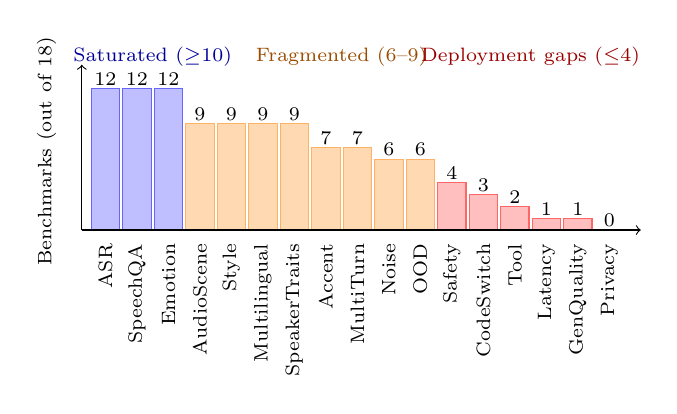
\begin{tikzpicture}[
  every node/.style={font=\footnotesize},
  bar/.style={fill=blue!25, draw=blue!60},
  bargap/.style={fill=orange!30, draw=orange!60},
  barlow/.style={fill=red!25, draw=red!60}
]
\foreach \i/\name/\count/\style in {
  1/ASR/12/bar,
  2/SpeechQA/12/bar,
  3/Emotion/12/bar,
  4/AudioScene/9/bargap,
  5/Style/9/bargap,
  6/Multilingual/9/bargap,
  7/SpeakerTraits/9/bargap,
  8/Accent/7/bargap,
  9/MultiTurn/7/bargap,
  10/Noise/6/bargap,
  11/OOD/6/bargap,
  12/Safety/4/barlow,
  13/CodeSwitch/3/barlow,
  14/Tool/2/barlow,
  15/Latency/1/barlow,
  16/GenQuality/1/barlow,
  17/Privacy/0/barlow
}{
  \ifnum\count>9
    \draw[bar] (\i*0.4-0.18,0) rectangle (\i*0.4+0.18, \count*0.15);
  \else\ifnum\count>4
    \draw[bargap] (\i*0.4-0.18,0) rectangle (\i*0.4+0.18, \count*0.15);
  \else
    \draw[barlow] (\i*0.4-0.18,0) rectangle (\i*0.4+0.18, \count*0.15);
  \fi\fi
  \node[rotate=90, anchor=east, font=\scriptsize] at (\i*0.4, -0.05) {\name};
  \node[font=\scriptsize] at (\i*0.4, \count*0.15+0.12) {\count};
}
\draw[->] (0.1,0) -- (7.2,0);
\draw[->] (0.1,0) -- (0.1,2.1);
\node[rotate=90, anchor=south, font=\scriptsize] at (-0.1,1.0) {Benchmarks (out of 18)};
\node[font=\scriptsize, blue!60!black]   at (1.0,2.2) {Saturated ($\geq$10)};
\node[font=\scriptsize, orange!60!black] at (3.4,2.2) {Fragmented (6--9)};
\node[font=\scriptsize, red!60!black]    at (5.8,2.2) {Deployment gaps ($\leq$4)};
\end{tikzpicture}
\caption{Capability coverage across 18 Speech LLM benchmarks
(2024--2026). Each bar shows how many benchmarks in our corpus
explicitly evaluate the capability. Coverage is dominated by ASR,
spoken question answering, and emotion; deployment-facing dimensions
(safety, code-switching, tool use, latency, generation quality,
privacy) remain weakly covered. The underlying 18~$\times$~17 coverage
matrix is released as supplementary material.}
\label{fig:benchmark_heatmap}
\end{figure}

The field is missing joint evaluation, not more benchmarks. A
capability may appear in several benchmarks while still being measured
under incompatible data sources, prompts, metrics, or judge protocols, and
the dimensions most needed for deployment (latency, safety, privacy,
generation quality) are precisely those least represented. We turn next to
whether even the dimensions that \emph{are} measured are measured
reliably.

\subsection{Methodological Validity: Data, Metrics, Judges, and Protocols}
\label{subsec:eval_validity}

The central issue is validity: whether a benchmark measures what it claims
to measure under conditions that support the conclusions being drawn. Four
forms of validity are especially relevant.

\paragraph{Construct validity.}
Construct validity asks whether the scoring method matches the target
capability. Multiple-choice formats, as in MMAU and AKB-2000
\cite{sakshi2024mmau,lu2026akb2000}, improve reproducibility but
underrepresent open-ended semantic behavior. Rule-based free-response
metrics such as WER, CER, F1, and ROUGE are objective but brittle under
paraphrase, script variation, and downstream task semantics. LLM-as-judge
scoring, used by AudioBench, VoiceBench, AIR-Bench, SD-Eval, and
SeaLLMs-Audio
\cite{wang2025audiobench,chen2024voicebench,yang2024airbench,ao2024sdeval,liu2025seallmsaudio},
better supports open-ended responses but introduces judge choice, prompt
sensitivity, and position-bias concerns formalized for text in
\cite{zheng2023judging}. SALMon \cite{maimon2024salmon} introduces a fifth
paradigm---modeling-based pairwise preference via likelihood
comparisons---that requires no external judge but is restricted to
relative comparisons. For subjective targets such as emotion and style,
single hard labels can be misleading because annotator disagreement is
part of the phenomenon. VoxEmo's distribution-aware metrics
\cite{zhang2026voxemo} therefore offer a principled direction for
paralinguistic evaluation, though the approach has so far been validated
on only two models (Qwen2-Audio and Audio Flamingo). The field needs
a second tier of metrics that match each capability's epistemic structure:
distributional for ambiguous targets, modeling-based for relative
comparison, and exact-match for pure information retrieval.

\paragraph{Ecological validity.}
Ecological validity asks whether benchmark data resembles real speech use.
Real recordings preserve speaker variability, disfluency, and spontaneous
acoustic artifacts, but they are costly and often have uneven demographic
coverage. Synthetic TTS data is scalable and controllable, enabling
benchmarks such as VoiceBench, StyleBench, VoiceAgentBench, and Audio2Tool
\cite{chen2024voicebench,zhao2026stylebench,jain2025voiceagentbench,pahwa2026audio2tool}
to cover many prompts or scenarios; however, synthetic speech may smooth
away idiosyncratic speaker behavior, fatigue, natural hesitation, and
real environmental variation. Hybrid designs that overlay perturbations
or scenes on real speech, as in SCENEBench and Hearing2Translate
\cite{iyer2026scenebench,papi2025hearing2translate}, are useful but still
require validation against natural recordings. We therefore propose
that synthetic-only benchmarks should not anchor deployment claims; any
fairness, robustness, or deployment claim should include a real-speech
validation slice.

\paragraph{Evaluator validity: judge agreement.}
Evaluator validity asks who or what judges the output. LLM judges make
large-scale open-ended evaluation feasible, but reported agreement with
humans is moderate rather than definitive. SD-Eval reports a Spearman
correlation $\rho = 0.613$ between GPT-4o judge scores and human ratings
\cite{ao2024sdeval}; SeaLLMs-Audio reports a Pearson correlation of 0.8
with 93\% agreement excluding ties \cite{liu2025seallmsaudio}; AIR-Bench
explicitly documents position bias and mitigates with answer-swap voting
\cite{yang2024airbench}; the canonical text-LLM judge-bias literature
\cite{zheng2023judging} confirms that these issues are systemic, not
benchmark-specific.

\paragraph{Evaluator validity: contamination risk.}
A more serious risk emerges when proprietary LLMs
help generate benchmark items, filter annotations, or score outputs. The
AKB-2000 paper \cite{lu2026akb2000} explicitly acknowledges that
proprietary LLMs co-curated its questions, capping their performance at
94--96\% as upper bound rather than independent measurement; FMSU-Bench
\cite{li2026fmsubench} uses Gemini 2.5 Pro as primary annotator with
multi-expert cross-validation; SeaLLMs-Audio uses Gemini-2.5-flash as
judge for the same model class. In each case a model's score may
partially reflect the curation pipeline rather than independent
capability. Human baselines remain limited: only three benchmarks in our
pool (MMAU, SD-Eval, SALMon) report human upper bounds at scale, making
it hard to interpret whether a given score indicates saturation,
progress, or metric artifact. We therefore propose that proprietary
judges should not score the same model family that helped curate the
benchmark, and that human baselines should accompany any new capability
claim.

\paragraph{Operational validity.}
Operational validity asks whether the benchmark reflects deployment. Many
benchmarks are valid for offline comparison but weak for choosing a
real-time voice assistant. Latency, streaming mode, endpointing, audio
chunking, hardware, batch size, interruption handling, and multi-turn
stability are rarely standardized alongside task accuracy. SCENEBench
\cite{iyer2026scenebench} is the only benchmark in the pool that
measures per-clip latency, and it does so in isolation from content
quality. VoiceAgentBench \cite{jain2025voiceagentbench} addresses tool
use but explicitly does not study dynamic real-time tool invocation.
This creates a deployment mismatch: benchmarks may report that a model
understands speech while remaining silent about whether it can respond
quickly, preserve paralinguistic cues, and remain safe during an
interactive session. We elaborate the latency and streaming dimensions
of this mismatch in Section~\ref{sec:deployment}. We therefore
propose that latency, streaming, and content quality should be jointly
reported, not separately.

\paragraph{Severity ranking.}
Among the four validity types, operational validity is the most damaging
for IPM-relevant deployment claims: a benchmark can score perfectly on
construct, ecological, and evaluator validity yet still fail to inform a
practitioner choosing a real-time voice system. Construct and evaluator
validity interact in direct tension---tightening one (e.g., requiring
distribution-aware scoring) often weakens the other (e.g., by demanding
LLM judges that cannot represent label distributions)---so they must be
balanced rather than maximized independently.

\subsection{Which Models Are Actually Evaluated? Reporting Bias and Deployment Mismatch}
\label{subsec:eval_models}

Existing benchmark surveys ask ``what does each benchmark cover?'' We
instead ask ``which models are systematically benchmarked, and which
remain invisible?'' The model-evaluation matrix concentrates around
accessible or widely recognized systems. Qwen2-Audio \cite{team2024qwen2}
appears in nine benchmarks; Whisper variants \cite{radford2023robust},
GPT-4o \cite{openai2024gpt4o}, and Whisper+LLM cascades each appear in
seven; Audio Flamingo \cite{kong2024audioflamingo} and Qwen2.5-Omni
\cite{xu2025qwen25omni} appear in six; SALMONN \cite{tang2023salmonn} and
LLaMA variants \cite{touvron2023llama} appear in five; pre-2.0 Qwen-Audio
\cite{bai2023qwen}, Gemini variants \cite{google2024gemini}, Qwen3-Omni
\cite{xu2025qwen25omni}, Mini-Omni \cite{xie2024miniomni}, Kimi-Audio
\cite{du2025kimiaudio}, and DeSTA2 \cite{lu2026desta2} each appear in
four. The concentration
is understandable: open-weight models are easier to run, Whisper cascades
serve as convenient baselines, and proprietary frontier models such as
GPT-4o and Gemini provide recognizable reference points.

This concentration creates reporting bias. Coverage of interaction-first
systems is sparse and asymmetric. Moshi \cite{défossez2024moshispeechtextfoundationmodel}
and the GPT-4o-Audio real-time mode each appear in a single benchmark
(VoiceBench \cite{chen2024voicebench}). Four other interaction-first
systems---MiniCPM-o 4.5, Voila, OmniFlatten, and Gemini Live
\cite{google2024gemini}---do not appear in any benchmark in our pool.
Ordinary GPT-4o or Gemini evaluations should be distinguished in
practice from evaluations of their real-time audio interaction
modes (the GPT-4o = 7 and Gemini = 4 counts in the matrix include
text-mode evaluations; real-time-audio-mode evaluation is essentially
absent from our pool). This is precisely the deployment regime that
motivates the Speech-LLM concept, and it is precisely the regime that
existing benchmarks fail to evaluate. We elaborate the deployment
implications of this gap in Section~\ref{sec:deployment}.

\subsection{Validity Gaps and Benchmark Design Principles}
\label{subsec:eval_gaps}

The four validity questions of Section~\ref{subsec:eval_validity} surface
four parallel gaps. The construct validity gap: benchmarks repeatedly
measure ASR, spoken QA, and emotion, but subjective and multi-channel
capabilities need metrics that preserve ambiguity and cross-channel
interaction. The ecological validity gap: synthetic data enables scale
but weakens real-world claims unless paired with real-speech validation.
The operational validity gap: latency, streaming, endpointing,
interruption handling, and multi-turn stability are not jointly
evaluated with content quality. The governance validity gap: safety,
privacy, speaker anonymity, provenance, and identity risks are
under-integrated into mainstream benchmark design and demand the
extended treatment in Section~\ref{sec:safety_privacy_governance}.

We propose five design principles for future Speech LLM benchmarks:

\begin{enumerate}
  \item \textbf{Multi-channel joint evaluation.} Each benchmark should
  report at least two of: content fidelity, paralinguistic awareness,
  interaction dynamics, latency, and safety. Audio2Tool's joint
  reporting of ASR, tool-use accuracy, and noise robustness
  \cite{pahwa2026audio2tool} is a partial precedent.
  \item \textbf{Distribution-aware scoring for subjective targets.}
  Emotion and style should use soft labels or distributional metrics
  when annotator disagreement is intrinsic, following VoxEmo's
  KLD/JSD/TVD template \cite{zhang2026voxemo}.
  \item \textbf{Cross-source validation.} Claims based mainly on
  synthetic speech should be replicated on real-speech subsets.
  SCENEBench's pairing of 16k synthetic and 20 natural validation
  clips \cite{iyer2026scenebench} illustrates the design pattern,
  though the natural-speech fraction remains negligibly small.
  \item \textbf{Mandatory evaluation metadata.} Reports should
  document prompts, judge model and version, decoding settings,
  hardware, audio chunking, streaming mode, and whether any LLM was
  used during data curation. Cross-domain work on model governance similarly suggests that validation artifacts should be assessed for stability rather than treated as one-off explanations, as shown by recent evidence on SHAP attribution instability in credit-risk modeling~\cite{lin2025shap}.
  \item \textbf{Speech-LLM Evaluation Cards.} Analogous to ML model
  cards \cite{mitchell2019modelcards}, each benchmark should publish
  a structured card declaring: (a) primary and secondary lenses from
  Table~\ref{tab:benchmark_taxonomy}; (b) capability cells from
  Figure~\ref{fig:benchmark_heatmap} that the benchmark measures;
  (c) data source (real, synthetic, hybrid); (d) scoring method
  (rule-based, LLM-judge with model and version, distribution-aware,
  modeling-based); (e) human baseline availability; (f) model
  coverage including any 0/$N$ omissions; and (g) acknowledged
  validity threats.
\end{enumerate}

\noindent Of these, Principle~1 is the most immediately actionable: it
requires no new dataset and can be retrofitted into current benchmark
releases by adding latency and safety metrics alongside existing
capability scores.

Evaluation is becoming a bottleneck for trustworthy Speech LLM
deployment. Current benchmarks reveal individual capabilities but
under-measure the interactions among speech content, timing,
paralinguistics, safety, and real-world use that voice systems must
handle simultaneously. The four validity gaps motivate the
deployment-oriented analysis in Section~\ref{sec:deployment} and the
safety-and-governance analysis in Section~\ref{sec:safety_privacy_governance}.
\FloatBarrier